% !TEX root = ../my-thesis.tex
%
\chapter{Numerical Tools in Uncertainty Quantification}
\label{sec:ntools}

\cleanchapterquote{Al bon mestri no i mancin i feris: cence di l\^or no si f\^as nuie, e ogni un al f\^as il so mist\^ir.}{Friulian Proverb}{}

\section{Introduction}
\label{sec:ntools:intro}

\gls{uq} is a multidisciplinary field that encompasses various techniques and methods to quantify and manage uncertainty in computational models. The computational tools used in \gls{uq} span a wide range of areas, including statistical inference, optimization, sensitivity analysis, and surrogate modeling. In this chapter, we do not aim to provide an exhaustive review of all the numerical tools used in UQ, but rather to introduce a subset of tools that have been repeatedly used in this thesis. These tools include \gls{gpr} to approximate the function distributions, \gls{mcmc} methods to sample unnormalized probability distributions, and \glspl{svm} for classification. We provide a brief overview of each of these tools, their underlying principles, and some useful properties that we used.

\smallskip
This chapter is inspired by the book \textit{Uncertainty Quantification: Theory, Implementation, and Applications} by Ralph C. Smith \cite{uq_theory}, which provides an excellent introduction to the field of UQ and covers a wide range of topics, including the numerical tools discussed in this chapter. We also refer the reader to other textbooks and resources for a more in-depth treatment of these tools, such as \textit{Gaussian Processes for Machine Learning} by Carl Edward Rasmussen and Christopher K. I. Williams \cite{gp_rasmussen} and \textit{Computational Statistics}, by Antti Honkela \cite{comp_stat}, which provides an excellent introduction to computational statistics. For the theory and algorithms of Support Vector Machines, we refer the reader to \textit{Statistical Pattern Recognition} by Andrew Webb \cite{stats_pr}.

\smallskip
Finally, all the numerical tools presented in this chapter, and many more, were implemented into the \texttt{CMP++} library, which is available as open-source software~\cite{CMP++} and was used to perform all the numerical experiments presented in this thesis. The library is implemented in \texttt{C++} and provides a wide range of basic functionalities for \gls{uq}, including regression, sampling, optimization, clustering and classification, as well as the more advanced algorithms presented in this thesis, such as the CMP method and the model-based clustering and piecewise regression method.


\section{Gaussian Process Regression}
\label{sec:ntools:gpr}

In this section, we introduce the concept of \gls{gpr}, which is a non-parametric regression method that allows practitioners to model complex relationships between input and output variables. After a brief introduction on regression, we will introduce the concept of \glspl{gp} and their properties, and then we will discuss how \glspl{gpr} can be used for regression tasks. We will also discuss some of the practical considerations when using \gls{gpr}, such as the choice of covariance functions and hyperparameter tuning, as well as some more advanced topics used in this thesis.

\subsection{What Is Regression?}
Given a set of observations $\mathcal{D} = \{(\bx_i, y_i)\}_{i=1}^{\nobs}$, where $\bx_i \in X \subset \reals^{d_x}$ is a vector of independent variables and $y_i \in Y \subset \reals$ is the corresponding dependent variable, regression aims to find a function $f(\bx)$ such that $y_i \approx f(\bx_i)$ for all $i$. 
Practitioners often restrict the space of candidate functions by introducing a parametric family of functions $F_{\btheta} = \{f(\bx; \btheta) : \btheta \in \Theta\}$, where $\btheta$ is a vector of parameters that define the function. The goal of regression is then to identify a specific function $f(\bx; \btheta^\star)$ from the parametric family that best fits the observed data, where $\btheta^\star$ is the optimal set of parameters. This is typically done by minimizing a loss function that measures the discrepancy between the predicted values and the observed values, such as the \gls{mse} or the negative log-likelihood. 

\smallskip
Another interesting approach to regression is \textit{non-parametric} regression, in which we specify a large function space $F$ that contains a wide range of possible functions, for example the space of all smooth functions $C^\infty(\Omega)$. Such a function space is usually richer than most parametric families, and allows us to model more complex relationships between the input and output variables. We then put a prior probability distribution, here termed as $\prior{f(\cdot)}$ over the function space $F$. Such a prior distribution encodes our prior beliefs about the function. Like any other random variable, we can draw realizations $f^{(\omega)} \sim \prior{f(\cdot)}$ from the prior distribution, which are random functions that represent possible realizations of the underlying function. When we observe data $\data$, we can update our beliefs about the function by conditioning the prior distribution on the observed data, which yields a posterior distribution $\mathrm{p}(f(\cdot) \mid \data)$. The posterior distribution represents our updated beliefs about the function after observing the data, and can be used to make predictions about the function values at new input points.

\begin{figure}[htbp]
\centering
% The resizebox ensures it fits perfectly on a beamer slide
\resizebox{\textwidth}{!}{%
\begin{tikzpicture}[
    % Global aesthetic settings
    font=\sffamily,
    >=Latex,
    % Style for the connecting arrow
    connectarrow/.style={->, line width=2mm, color=gray!40, shorten >=5pt, shorten <=5pt},
    arrowlabel/.style={midway, above, font=\bfseries\large, color=black!70, align=center, yshift=5pt},
    % Style for plot axes to keep them clean
    myaxis/.style={
        width=7cm, height=5cm,
        axis lines=left,
        % --- These are the key settings to remove numbers and labels ---
        xlabel={}, % Remove x-axis label
        ylabel={}, % Remove y-axis label
        xtick=\empty, % Remove x-axis ticks and numbers
        ytick=\empty, % Remove y-axis ticks and numbers
        % ------------------------------------------------------------
        ymin=-3, ymax=3,
        xmin=0, xmax=6,
        domain=0:6, samples=100, no markers,
        axis line style={-},
    }
]

    % ====== LEFT PLOT: GP PRIOR ======
    \begin{axis}[
        myaxis,
        name=priorplot,
        title={Random Functions from a Prior Distribution.},
    ]
        % Draw a few simple, smooth random realizations manually
        % for a very clean "simple" look.
        \addplot[black, very thick, smooth, tension=1] coordinates {(0,1) (2,-1.5) (4,2) (6,0)};
        \addplot[black, very thick, smooth, tension=1] coordinates {(0,-0.5) (3,1) (5,-2) (6,-0.5)};
        \addplot[black, very thick, smooth, tension=0.8] coordinates {(0,-2) (1.5,0) (4,-1) (6,1.5)};
        \addplot[black, very thick, smooth, tension=0.9] coordinates {(0,1.5) (2,2) (4,-0.5) (6,-2)};
        \addplot[black, very thick, smooth, tension=0.7] coordinates {(0,0) (2,0.5) (4,-0.5) (6,0)};
    \end{axis}


    % ====== RIGHT PLOT: GP POSTERIOR ======
    % Shifted to the right by 9cm
    % ====== RIGHT PLOT: GP POSTERIOR ======
    \begin{axis}[
        myaxis,
        at={(9cm,0)}, 
        name=postplot,
        title={Random Functions from a Posterior Distribution.},
    ]
        % --- Target Data Points (for reference) ---
        % D1: (1.5, 1.2) | D2: (3.5, -0.8) | D3: (5.0, 0.5)
        
        % --- Realisation 1 (Red) ---
        % Passes near the points, wiggles in between
        \addplot[black, very thick, smooth, tension=0.6] coordinates {
            (0, 0.5) (1.5, 1.3) (2.5, 0.2) (3.5, -0.7) (5.0, 0.6) (6, 0.2)
        };

        % --- Realisation 2 (Teal) ---
        % Starts lower, intersects, ends lower
        \addplot[black, very thick, smooth, tension=0.7] coordinates {
            (0, -0.5) (1.5, 1.1) (2.5, -0.2) (3.5, -0.9) (5.0, 0.4) (6, -0.5)
        };

        % --- Realisation 3 (Orange) ---
        % Different wiggle pattern
        \addplot[black, very thick, smooth, tension=0.8] coordinates {
            (0, 1.5) (1.5, 1.25) (2.5, 0.8) (3.5, -0.85) (5.0, 0.55) (6, 1.2)
        };


        % --- Data Points with Error Bars (Drawn on top) ---
        \addplot+[
            only marks, 
            mark=*, mark size=3pt, mark options={fill=white, draw=red, line width=1pt},
            error bars/.cd, 
            y dir=both, y fixed=0.3, 
            x dir=both, x fixed=0.3, 
            error bar style={red, very thick}
        ] coordinates {
            (1.5, 1.2)
            (3.5, -0.8)
            (5.0, 0.5)
        };
        
    \end{axis}


    % ====== CONNECTING ARROW ======
    % Draw arrow between the two axis environments
    \draw[connectarrow] ($(priorplot.east)+(0.2,0)$) -- 
                        node[arrowlabel] {} 
                        ($(postplot.west)+(-0.2,0)$);

\end{tikzpicture}
} % End resizebox
\caption{Left: A Random Distribution over Functions. Right: A Random Distribution over Functions Conditioned on Data. The data points are shown with error bars.}
\label{fig:ntools:gp_prior_posterior}
\end{figure}

In Fig.~\ref{fig:ntools:gp_prior_posterior}, we illustrate the main ideas behind non-parametric regression. On the left, we show some random realizations of a function, which should be thought of as a random sample from a prior distribution over functions. On the right, we show some random realizations of a function conditioned on a set of observations (shown as red points with error bars). The realizations on the right are drawn from the posterior distribution over functions, which is obtained by conditioning the prior distribution on the observed data. 

\smallskip
The power of non-parametric regression lies in its ability to model complex relationships between the input and output variables without the need to specify a parametric form for the function. Furthermore, non-parametric regression provides a natural way to quantify uncertainty in the predictions, as the posterior distribution over functions can be used to compute confidence intervals and make probabilistic statements about the function values at new input points. In the next section, we will introduce \glspl{gp}, which assume that the prior distribution over functions is a \gls{gp}, and discuss how \glspl{gp} can be used for regression tasks.


\subsection{Introduction to Gaussian Processes}
A \gls{gp} is a collection of random variables, any finite number of which have a joint Gaussian distribution. According to our previous discussion, a \gls{gp} can be thought of as a probability distribution over functions. This distribution is fully specified by a mean function $m(\bx)$ and a covariance function $k(\bx, \bx')$, which define the mean and covariance of the function values at any two points $\bx$ and $\bx'$. The mean function $m(\bx)$ represents the expected value of the function at point $\bx$, while the covariance function $k(\bx, \bx')$ represents the degree of similarity between the function values at points $\bx$ and $\bx'$. The mean and covariance functions are typically parameterized by a set of hyperparameters $\bpsi$, and will be denoted as $m_{\bpsi}(\bx)$ and $k_{\bpsi}(\bx, \bx')$ to make this dependence explicit. 

\smallskip
In this thesis, we define a \gls{gp} distribution as follows:

\begin{equation}
  f(\bx) \sim\mathcal{GP}(m_{\bpsi}(\bx), k_{\bpsi}(\bx, \bx')).
   \label{eq:gp_definition}
\end{equation}

\smallskip
The covariance function $k_{\bpsi}(\bx, \bx')$ is said to be stationary if it can be expressed as function of the lag $\mathbf{r} = \bx - \bx'$ between the two input points. Practitioners often use stationary covariance functions and assume a zero mean prior function. In this case, the hyperparameters $\bpsi$ are the parameters of the covariance function, such as the length scale and variance parameters. Some commonly used covariances include the \gls{rbf} covariance, the Mat\'ern $5/2$ covariance, and the Mat\'ern $1/2$ covariance. The choice of the covariance function and its hyperparameters can have a significant impact on the properties of the \gls{gp} and the resulting function realizations.

\begin{figure}
  \centering
  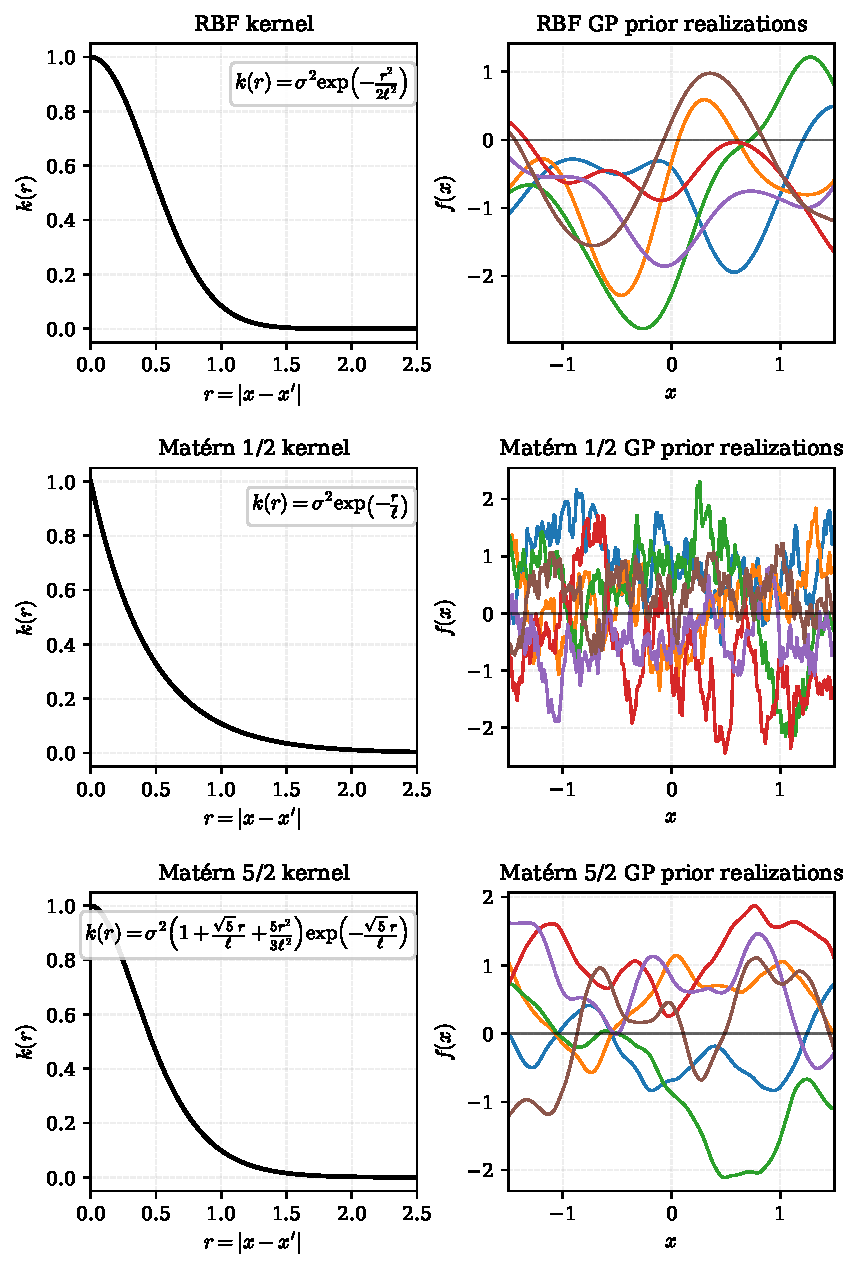
\includegraphics[width=0.95\linewidth]{figures/numtools/gp_kernels_priors.pdf}
  \caption{Left column: profiles of $k(r)$ for \gls{rbf}, Mat\'ern $5/2$, and Mat\'ern $1/2$. Right column: sample realizations from the corresponding \gls{gp} priors.}
  \label{fig:ntools:gp_kernels_priors}
\end{figure}

\begin{figure}
  \centering
  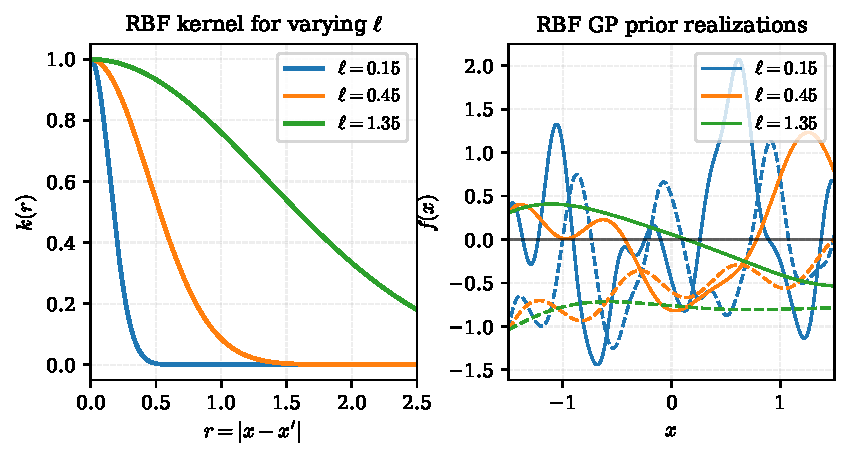
\includegraphics[width=0.95\linewidth]{figures/numtools/rbf_lengthscales.pdf}
  \caption{Left column: profiles of $k(r)$ for \gls{rbf} covariance with different length scales. Right column: sample realizations from the corresponding \gls{gp} priors.}
  \label{fig:ntools:gp_kernels_lengthscale}
\end{figure}

This is illustrated in Fig.~\ref{fig:ntools:gp_kernels_priors}, where we show the covariance profiles (left) and sample realizations (right) from the corresponding \gls{gp} priors for the \gls{rbf}, Mat\'ern $5/2$, and Mat\'ern $1/2$ covariances. The profiles show how the covariance between function values at two points decays as the distance between the points increases. \gls{rbf} covariances yield functions that are infinitely differentiable, while Mat\'ern covariances yield functions that are only $n$-times differentiable, where $n$ is determined by the choice of the Mat\'ern covariance. For example, the Mat\'ern $5/2$ covariance yields functions that are twice differentiable, while the Mat\'ern $1/2$ covariance yields functions that are not differentiable. In Fig.~\ref{fig:ntools:gp_kernels_lengthscale}, we show the effect of the length scale hyperparameter on the covariance profile and the resulting function realizations for the \gls{rbf} covariance. As the length scale increases, the covariance becomes wider and the resulting functions become more or less variable (points are more correlated across the input space), while as the length scale decreases, the covariance becomes narrower and the resulting functions become more variable (points are less correlated across the input space).

\smallskip
To draw prior realizations on an input set
$\mathbf{X}=\{x_i\}_{i=1}^{\nobs}$ we should first build the covariance matrix
$k_{\bpsi}(\mathbf{X}, \mathbf{X})$ and mean vector $m_{\bpsi}(\mathbf{X})$. The prior distribution of the function values $\mathbf{f} = [f(\bx_1), \ldots, f(\bx_{\nobs})]^\top$ at the input points $\mathbf{X}$ is then given by a multivariate Gaussian distribution:
\[
\mathbf{f}\sim\mathcal{N}{(m_{\bpsi}(\mathbf{X}),k_{\bpsi}(\mathbf{X}, \mathbf{X}))}.
\]

To draw from this distribution, we must compute $k_{\bpsi}(\mathbf{X}, \mathbf{X})^{1/2}$, and draw a standard normal vector $\mathbf{z}\sim\mathcal{N}{(\mathbf{0},\mathbf{I})}$. A random realization is then obtained as $\mathbf{f}^{(\omega)} = m_{\bpsi}(\mathbf{X}) + k_{\bpsi}(\mathbf{X}, \mathbf{X})^{1/2}\mathbf{z}^{(\omega)}$.

\smallskip
To compute the \gls{gp} posterior distribution given a set of observations $\mathcal{D} = \{(\bx_i, y_i)\}_{i=1}^{\nobs}$ we can rely on the fact that the posterior distribution is also a \gls{gp}. Indeed, the joint distribution of the observed values $\mathbf{y} = [y_1, \ldots, y_{\nobs}]^\top$ and the function value at a new input point $\bx$, $f = f(\bx)$ is given by:

\begin{equation}
  \begin{bmatrix}
    \mathbf{y} \\
    f \\
  \end{bmatrix} \sim \mathcal{N}\left(
  \begin{bmatrix}
    m_{\bpsi}(\mathbf{X}) \\
    m_{\bpsi}(\bx) \\
  \end{bmatrix},
  \begin{bmatrix}
    k_{\bpsi}(\mathbf{X}, \mathbf{X}) + \sigma^2\mathbf{I} & k_{\bpsi}(\mathbf{X}, \bx) \\
    k_{\bpsi}(\bx, \mathbf{X}) & k_{\bpsi}(\bx, \bx)
  \end{bmatrix}\right)\;,
  \label{eq:gp_joint_distribution}
\end{equation}

where $\sigma^2$ is the variance of the observation noise. Using the block matrix inversion lemma, we can compute the conditional mean and covariance of the resulting conditional distribution,

\begin{equation}
  \begin{aligned}
    m_{\bpsi}(\bx \mid \mathcal{D}) &= m_{\bpsi}(\bx) + k_{\bpsi}(\bx, \mathbf{X})^\top[k_{\bpsi}(\mathbf{X}, \mathbf{X}) + \sigma^2\mathbf{I}]^{-1}(\mathbf{y} - m_{\bpsi}(\mathbf{X}))\;, \\
    k_{\bpsi}(\bx, \bx' \mid \mathcal{D}) &= k_{\bpsi}(\bx, \bx^\prime) - k_{\bpsi}(\bx, \mathbf{X})^\top[k_{\bpsi}(\mathbf{X}, \mathbf{X}) + \sigma^2\mathbf{I}]^{-1}k_{\bpsi}(\bx^\prime,\mathbf{X})\;.
  \end{aligned}
  \label{eq:gp_posterior_gp}
\end{equation}

For notational simplicity, we will often refer to the posterior distribution of the \gls{gp} as $\mathcal{GP}(m_{\bpsi}, k_{\bpsi} \mid \data)$.

\subsection{Hyperparameter Selection Via Maximum Marginal Likelihood}
\label{sec:ntools:gpr:mml}

The hyperparameters $\bpsi$ of the \gls{gp}, including the parameters of the covariance function and the observation noise variance $\sigma^2$, play a crucial role in determining the behavior of the model, as evident from Fig.~\ref{fig:ntools:gp_kernels_lengthscale}. Rather than specifying these hyperparameters manually, we can optimize them directly from the data by maximizing the marginal likelihood (also known as the evidence) of the observations.

\smallskip
The marginal likelihood is obtained by integrating out the function values $\mathbf{f}$ from the joint distribution of the observations and the function:

\begin{equation}
  \mathrm{p}(\mathbf{y} \mid \mathbf{X}, \bpsi, \sigma^2) = \int \mathrm{p}(\mathbf{y} \mid \mathbf{f}, \sigma^2) \mathrm{p}(\mathbf{f} \mid \mathbf{X}, \bpsi) \dd\mathbf{f}\;.
\end{equation}

For a \gls{gp} prior with a Gaussian likelihood, this marginal likelihood is available in closed form:

\begin{equation}
  \mathrm{p}(\mathbf{y} \mid \mathbf{X}, \bpsi, \sigma^2) = \mathcal{N}(\mathbf{y}; m_{\bpsi}(\mathbf{X}), k_{\bpsi}(\mathbf{X}, \mathbf{X}) + \sigma^2\mathbf{I})\;,
  \label{eq:marginal_likelihood}
\end{equation}

which can be written in terms of its log-form as:

\begin{equation}
\begin{split}
  \log \mathrm{p}(\mathbf{y} \mid \mathbf{X}, \bpsi, \sigma^2) & = -\frac{1}{2}(\mathbf{y} - m_{\bpsi}(\mathbf{X}))^\top\mathbf{K}^{-1}(\mathbf{y} - m_{\bpsi}(\mathbf{X})) \\
  & \quad - \frac{1}{2}\log\det(\mathbf{K}) - \frac{\nobs}{2}\log(2\pi)\;,
\end{split}
  \label{eq:log_marginal_likelihood}
\end{equation}

where $\mathbf{K} = k_{\bpsi}(\mathbf{X}, \mathbf{X}) + \sigma^2\mathbf{I}$ is the covariance matrix of the observations.

\smallskip
The optimal hyperparameters can be found by maximizing the log-marginal likelihood with respect to $\bpsi$:

\begin{equation}
  \bpsi^\star = \argmax_{\bpsi}\; \log \mathrm{p}(\mathbf{y} \mid \mathbf{X}, \bpsi, \sigma^2)\;.
  \label{eq:hyperparameter_optimization}
\end{equation}

This approach is called the \gls{mml} method. The first term in Eq.~\eqref{eq:log_marginal_likelihood} represents the data fit, while the second term acts as an automatic regularization that penalizes model complexity, effectively preventing overfitting. The gradients of the log-marginal likelihood with respect to the hyperparameters are available in closed form~\cite{gp_rasmussen}.

\subsection{Evaluating a Random Realization of a Gaussian Process}
\label{sec:ntools:constr}

The posterior mean and variance of the \gls{gp} at a new input point $\bx$ can be computed using Eq.~\eqref{eq:gp_posterior_gp}. Notice that both the posterior mean and variance can be evaluated parametrically at any point $\bx$. The same cannot be said for a random realization of the \gls{gp}, which can only be evaluated at a finite set of input points $\mathbf{X}$. 

\smallskip
Being able to evaluate a random realization of a \gls{gp}, here termed $f^{(\omega)}(\bx)$, at any point $\bx$ is important for many applications, and we will present one in \S\ref{sc:surr:candidate}. In this section, we present an efficient method to compute a parametric representation of a random realization of a \gls{gp} based on the idea of interpolating it with the same \gls{gp} used to generate it.

\smallskip
We start by drawing a random realization of the posterior \gls{gp} at an evaluation set, $\mathbf{X}_e = \{\bx_e^i\}_{i=1}^{\neval}$, which corresponds to a random vector $\mathbf{f}_e^{(\omega)}$:

\begin{equation}
    \mathbf{f}_e^{(\omega)} = m_{\bpsi}(\mathbf{X}_e \mid \data) + k_{\bpsi}(\mathbf{X}_e, \mathbf{X}_e \mid \data)^{1/2} \mathbf{z}^{(\omega)}\;,
\label{eq:pred_mean_e}
\end{equation}

where $\mathbf{z}^{(\omega)} \sim \mathcal{N}(\mathbf{0}, \mathbf{I})$. We use this random vector $\mathbf{f}_e^{(\omega)}$ as a set of pseudo-observations to augment the original observation set $\mathcal{D}$ into a new observation set $\mathcal{D}_{+}^{(w)} = \mathcal{D} \cup \{(\bx_e^i, f_{e,i}^{(\omega)})\}_{i=1}^{\neval}$, where $f_{e,i}^{(\omega)}$ is the $i$-th component of the random vector $\mathbf{f}_e^{(\omega)}$. We can now use this augmented observation set $\mathcal{D}_{+}^{(w)}$ to compute the posterior distribution of the \gls{gp} at any point $\bx$ using the standard \gls{gp} regression equations (keeping the same hyperparameters $\bpsi$). The mean of this posterior distribution at point $\bx$ is given by:

\begin{equation}
\begin{split}
    m_{\bpsi}(\bx \mid \mathcal{D}_{+}^{(w)}) & = m_{\bpsi}(\bx \mid \data) + \begin{bmatrix} k_{\bpsi}(\bx, \mathbf{X}) \\ k_{\bpsi}(\bx, \mathbf{X}_e) \end{bmatrix}^{\top} \begin{bmatrix} k_{\bpsi}(\mathbf{X}, \mathbf{X}) & k_{\bpsi}(\mathbf{X}, \mathbf{X}_e)^{\top} \\ k_{\bpsi}(\mathbf{X}_e, \mathbf{X}) & k_{\bpsi}(\mathbf{X}_e, \mathbf{X}_e) \end{bmatrix}^{-1} \\
    & \times \begin{bmatrix} \mathbf{y} - m_{\bpsi}(\mathbf{X}) \\ \mathbf{f}_e^{(\omega)} - m_{\bpsi}(\mathbf{X}_e) \end{bmatrix}\;.
\end{split}
\label{eq:pred_mean_x}
\end{equation}

Note that Eq.~\eqref{eq:pred_mean_x} can be further simplified using Eq.~\eqref{eq:pred_mean_e} and the block-matrix inversion formulae and becomes,

\begin{equation}
    \left.
    \begin{aligned}
      &m_{\bpsi}(\bx \mid \mathcal{D}_{+}^{(w)}) = m_{\bpsi}(\bx \mid \data) + k_{\bpsi}(\bx, \mathbf{X}_e) \boldsymbol{\alpha}_e^{(\omega)} - k_{\bpsi}(\bx, \mathbf{X}) \boldsymbol{\alpha}_o^{(\omega)}\;.\\
      &\boldsymbol{\alpha}_e^{(\omega)} = k_{\bpsi}(\mathbf{X}_e, \mathbf{X}_e \mid \data)^{-1/2} \mathbf{z}^{(\omega)}\;.\\
      &\boldsymbol{\alpha}_o^{(\omega)} =  k_{\bpsi}(\mathbf{X}, \mathbf{X})^{-1}k_{\bpsi}(\mathbf{X}, \mathbf{X}_e) k_{\bpsi}(\mathbf{X}_e, \mathbf{X}_e \mid \data)^{-1/2} \mathbf{z}^{(\omega)}\;.
    \end{aligned}
    \right.
\label{eq:pred_mean_x_simp}
\end{equation}

Eq.~\eqref{eq:pred_mean_x} can be evaluated parametrically at any point $\bx$ at a cost of $\mathcal{O}(\neval+ \nobs)$, (by precomputing $\boldsymbol{\alpha}_e^{(\omega)}$ and $\boldsymbol{\alpha}_o^{(\omega)}$) and returns a random realization of the \gls{gp} at point $\bx$. Note that the evaluation of this random realization depends on the choice of the evaluation set $\mathbf{X}_e$. In particular, if the evaluation set $\mathbf{X}_e$ is well spread across the input space, then the resulting random realization will be able to capture the behavior of the \gls{gp} across the entire input space. On the other hand, if the evaluation set $\mathbf{X}_e$ is concentrated in a small region of the input space, then the resulting random realization will only be able to capture the behavior of the \gls{gp} in that region and will return to the posterior mean in regions not covered by the evaluation set.


{
\begin{figure}[htbp]
  \centering
  \begin{subfigure}[t]{0.49\linewidth}
    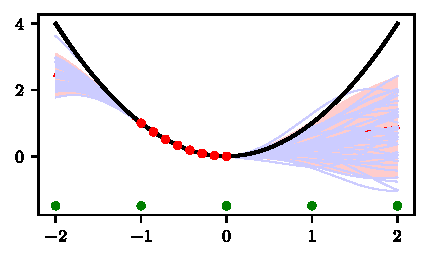
\includegraphics[width=\linewidth]{figures/surr/fig_a1.pdf}
    \caption{Case 1. Well spread evaluation set.}
    \label{fig:fig_a1}
  \end{subfigure}
  \begin{subfigure}[t]{0.49\linewidth}
    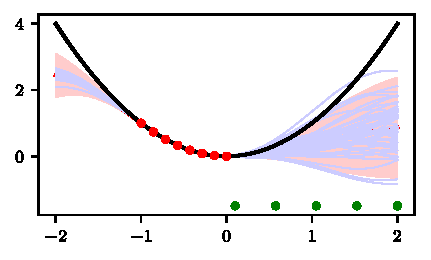
\includegraphics[width=\linewidth]{figures/surr/fig_a2.pdf}
    \caption{Case 2. Concentrated evaluation set.}
    \tikzmarknode{B}{}
    \label{fig:fig_a2}
  \end{subfigure}
  \centering
  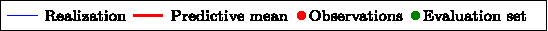
\includegraphics[width=0.7\linewidth]{figures/surr/fig_a3.pdf}
    \caption{Example of an interpolation of realizations of a GP using Eq.~\eqref{eq:pred_mean_x_simp}. Shaded areas represent the 95\% confidence interval.}
    \label{fig:fig_a}
\end{figure}
}


In Fig.~\ref{fig:fig_a} we show a simple example of Eq.~\eqref{eq:pred_mean_x_simp}. The chosen \gls{gp} has constant mean and squared exponential covariance function. The observations correspond to 8 points in the interval $[-1, 0]$ which follow a quadratic relationship, $y=x^2$. In both graphs we show the predictive mean and the 95\% confidence interval as well as 50 realizations evaluated using Eq.~\eqref{eq:pred_mean_x_simp}. In the left graph, the evaluation set $\mathbf{X}_e$ is well spread across the input space, and the resulting realizations are able to capture the behavior of the \gls{gp} across the entire input space, and we see that realizations cover the whole predictive variance interval. In the right graph, the evaluation set $\mathbf{X}_e$ is concentrated in a small region of the input space, and the resulting realizations are only able to capture the behavior of the \gls{gp} in that region, while they return close to the predictive mean in regions not covered by the evaluation set.

\subsection{Variance Reduction}
\label{sec:ntools:evr}

In this section we describe a useful property of the posterior \gls{gp} distribution, the \gls{evr} property. Such a property states that the reduction in posterior variance at a point $\bx$ induced by observing a new set of points $\data$ is always non-negative and is independent of the observed values $\mathbf{y}$. In other words, the posterior variance at a point $\bx$ after observing a new set of points $\data$ is always less than or equal to the prior variance at that point:

\begin{equation}
  \mathbb{V}_{\omega}[f^{(\omega)}(\bx) \mid \data] \leq \mathbb{V}_{\omega}[f^{(\omega)}(\bx)]\;.
\end{equation}

Furthermore, we can know in advance the amount by which the variance will be reduced at a point $\bx$ after observing a new set of points $\data$, without having to observe the corresponding function values. This property is evident from the expression for the posterior variance in Eq.~\eqref{eq:gp_posterior_gp}, which shows that the posterior variance at a point $\bx$ depends only on the covariance function $k_{\bpsi}$ and the locations of the observed points $\mathbf{X}$, but not on the observed values $\mathbf{y}$.

\smallskip
The \gls{evr} property is particularly useful in the context of active learning and Bayesian optimization, where we want to select new observation points to be added to the dataset that will lead to the greatest reduction in uncertainty about the function. We now seek a formula for the expected variance reduction at a point $\bx$ given that we will observe some new evaluation points $\mathbf{X}_e = \{\bx_e^i\}_{i=1}^{\neval}$, but having not yet observed the corresponding function values (except for the already observed data $\data$). Assuming the hyperparameters $\bpsi$ are fixed, the posterior variance at point $\bx$ after observing the new points $\mathbf{X}_e$ and $\mathbf{X}$ is given by:

\begin{equation}
\begin{split}
  \mathbb{V}_{\omega}[f^{(\omega)}(\bx) \mid \mathbf{X}_e \cup \mathbf{X}] & = k_{\bpsi}(\bx, \bx) - \begin{bmatrix}
    k_{\bpsi}(\bx, \mathbf{X}) \\
    k_{\bpsi}(\bx, \mathbf{X}_e)
  \end{bmatrix}^{\top} \begin{bmatrix}
    k_{\bpsi}(\mathbf{X}, \mathbf{X}) & k_{\bpsi}(\mathbf{X}, \mathbf{X}_e)^{\top} \\
    k_{\bpsi}(\mathbf{X}_e, \mathbf{X}) & k_{\bpsi}(\mathbf{X}_e, \mathbf{X}_e)
  \end{bmatrix}^{-1} \\
  & \times \begin{bmatrix}
    k_{\bpsi}(\mathbf{X}, \bx) \\
    k_{\bpsi}(\mathbf{X}_e, \bx)
  \end{bmatrix}\;.
\end{split}
\end{equation}

Using the block-matrix inversion formulae, we can derive a closed form expression for the variance reduction $\Delta \mathbb{V}_{\omega}(f^{(\omega)}(\bx) \mid \mathbf{X}_e)$ that does not require inverting the augmented covariance matrix:

\begin{equation}
\left.
\begin{aligned}
    &\Delta \mathbb{V}_{\omega}(f^{(\omega)}(\bx) \mid \mathbf{X}_e) = \boldsymbol{\rho}^{\top} k_{\bpsi}(\mathbf{X}_e, \mathbf{X}_e \mid \data)^{-1} \boldsymbol{\rho}\;,\\
    &\boldsymbol{\rho} = k_{\bpsi}(\mathbf{X}_e, \bx) - k_{\bpsi}(\mathbf{X}_e, \mathbf{X}) k_{\bpsi}(\mathbf{X}, \mathbf{X})^{-1} k_{\bpsi}(\mathbf{X}, \bx)\;.
\end{aligned}
\right.
\end{equation}

Assuming that $\neval << \nobs$, the computational cost of evaluating the expected variance reduction is $\mathcal{O}(\nobs^2)$, which is cheaper than the cost of having to invert the augmented covariance matrix, which is $\mathcal{O}((\nobs + \neval)^3)$.

\section{Markov Chain Monte Carlo}
\label{sec:ntools:mcmc}

\gls{mc} methods are a class of computational algorithms that rely on random sampling to estimate numerical quantities. They are without doubt the most widely used numerical tools in \gls{uq}, since they are essential for the estimation of integrals, optimization, and sampling from complex probability distributions. In this section, we focus on the use of \gls{mc} methods for estimating integrals and sampling from complex probability distributions.

\subsection{Monte Carlo Estimation of Integrals}
\label{sec:ntools:mcmc:mc}

The core of \gls{uq} is the estimation of integrals of the form:

\begin{equation}
  I = \int_{\Omega} f(\bx)\, \mathbb{P}(\dd \bx)\;,
  \label{eq:integral}
\end{equation}

where $f(\bx): \Omega \subset \reals^d \to \reals$ is a function of interest and $\mathbb{P}( \cdot)$ is a probability measure on the domain $\Omega$. These integrals are often denoted with the expectation notation $\mathbb{E}[f(\bx)]$ and are used to compute various quantities of interest in \gls{uq}, such as the mean, variance, and higher-order moments of a random variable, as well as the probability of certain events.

\smallskip
In this work, we consider cases where the measure $\mathbb{P}(\cdot)$ admits a density with respect to the Lebesgue measure, which we denote as $\pi(\bx)$. In this case, the integral in Eq.~\eqref{eq:integral} can be rewritten as:

\begin{equation}
  I = \int_{\Omega} f(\bx)\ \pi(\bx)\, \dd\bx\;.
  \label{eq:integral_density}
\end{equation}

While standard numerical integration methods, such as quadrature rules, can be used to estimate the integral in Eq.~\eqref{eq:integral_density} when the dimension of the domain $\Omega$ is low, they become computationally infeasible as the dimension increases due to the curse of dimensionality. \gls{mc} methods provide a powerful alternative for estimating these integrals, especially in high-dimensional spaces. The basic idea behind \gls{mc} methods is to draw random samples from the distribution $\prior{\bx}$ and use these samples to estimate the integral. Specifically, if we can draw $N$ samples $\{\bx_i\}_{i=1}^N$ from the distribution $\prior{\bx}$, we can estimate the integral as:

\begin{equation}
  \hat{I} = \frac{1}{N} \sum_{i=1}^N f_i\;.
  \label{eq:mc_estimate}
\end{equation}

Where $f_i = f(\bx_i)$ is the value of the function $f$ at the sample point $\bx_i$. The estimator $\hat{I}$ is an unbiased estimator of the integral $I$, and its variance decreases as $N$ increases, making it a consistent estimator. In fact, the MC estimator has several desirable properties, derived from the \gls{clt}:

\begin{itemize}
  \item Unbiasedness: $\mathbb{E}[\hat{I}] = I$.
  \item Consistency: $\hat{I} \xrightarrow{P} I$ as $N \to \infty$.
  \item Asymptotic normality: $\sqrt{N}(\hat{I} - I) \xrightarrow{d} \mathcal{N}(0, \sigma^2)$ as $N \to \infty$, where $\sigma^2 = \mathbb{V}_{\bx \sim \prior{\bx}}[f(\bx)]$ is the variance of $f(\bx)$ under the distribution $\prior{\bx}$.
\end{itemize}

Unfortunately, the asymptotic normality property of the \gls{mc} estimator also requires the samples $f_i$ to be independent. In practice, these samples are often correlated (we shall see in the next section why) and, while the asymptotic distribution remains normal, the variance of the estimator is higher. It is therefore important to be able to quantify the effect of this correlation on the variance of the \gls{mc} estimator and the parameters that govern it. 

\smallskip
Using Eq.~\eqref{eq:mc_estimate}, we can derive the variance of the \gls{mc} estimator as follows:

\begin{equation}
  \begin{aligned}
    \mathbb{V}[\hat{I}] &= \mathbb{E}\left[(\hat{I} - I)^2\right] \\
    &= \mathbb{E}\left[\frac{1}{N^2} \sum_{i=1}^N \tilde{f}_i\sum_{j=1}^N \tilde{f}_j \right] \\
  \end{aligned}
\end{equation}

Where $\tilde{f}_i = f_i - I$ is the centered version of the samples. Using the binomial expansion, we can simplify the formula as follows:

\begin{equation}
  \begin{aligned}
    \mathbb{V}[\hat{I}] &= \frac{1}{N^2} \sum_{i=1}^N \sum_{j=1}^N \mathbb{E}[\tilde{f}_i \tilde{f}_j] \\
    &= \frac{1}{N^2} \left( N\mathbb{E}[\tilde{f}_1^2] + 2\sum_{i=1}^{N-1}\sum_{j=i+1}^N \mathbb{E}[\tilde{f}_i \tilde{f}_j] \right) \\
    &= \frac{\sigma^2}{N} + \frac{2}{N^2}\sum_{i=1}^{N-1}\sum_{j=i+1}^N  \mathrm{Cov}(f_i, f_j)\;.
  \end{aligned}
\end{equation}

We see that if the samples $f_i$ are independent, i.e. $\mathrm{Cov}(f_i, f_j) = 0$ for $i \neq j$, then the variance of the \gls{mc} estimator reduces to $\mathbb{V}[\hat{I}] = \sigma^2 / N$. However, in the worst case scenario where the samples are perfectly correlated, i.e. $\mathrm{Cov}(f_i, f_j) = \sigma^2$ for all $i \neq j$, then the variance of the \gls{mc} estimator reduces to $\mathbb{V}[\hat{I}] = \sigma^2$ and does not decrease with $N$. In general, we can expect the covariance between the samples to exponentially decay as the distance between the samples increases,

\begin{equation}
  \mathrm{Cov}(f_i, f_j) = \sigma^2 \exp \left(-\dfrac{|k|}{\ell}\right)\;,
\end{equation}

where $k = j - i$ is the distance between the samples and $\ell$ is a characteristic length scale that governs the rate of decay of the covariance. This last quantity is very important and we shall see in the next section how to estimate it.

\smallskip
Substituting this expression for the covariance into the formula for the variance, we get:

\begin{equation}
  \begin{aligned}
    \mathbb{V}[\hat{I}] &= \frac{\sigma^2}{N} + \frac{2\sigma^2}{N^2}\sum_{i=1}^{N-1}\sum_{j=i+1}^N \exp \left(-\dfrac{|j - i|}{\ell}\right) \\
    &= \frac{\sigma^2}{N^2} \left[ \dfrac{N(1-\rho^2) -2\rho(1-\rho^N)}{(1-\rho)^2}\right]\\
    &\approx \frac{\sigma^2}{N} \left[ \dfrac{1+\rho}{1-\rho}\right]\;.
  \end{aligned}
  \label{eq:ess}
\end{equation}

Where $\rho = \exp(-1/\ell)$ is the lag-1 autocorrelation of the samples and the last approximation holds if $\rho^n << 1$ (hence $N >> \ell$). This allows us to define an effective sample size $N_{\mathrm{eff}} = N \frac{1-\rho}{1+\rho}$, which allows us to quantify the variance of the \gls{mc} estimator in the presence of correlated samples as $\mathbb{V}[\hat{I}] \approx \sigma^2 / N_{\mathrm{eff}}$. 

\smallskip
As an example, we consider the estimation of the square of a random variable $x \sim \mathcal{N}(0, 1)$ using the \gls{mc} estimator in Eq.~\eqref{eq:mc_estimate}. We generate $N = 10^4$ samples from the distribution of $x$ and compute the \gls{mc} estimator $\hat{I} = \frac{1}{N} \sum_{i=1}^N x_i^2$. Notice that the true value of the integral is $I = \mathbb{E}[x^2] = 1$ while its variance is $\mathbb{V}[x^2] = 2$. We study how the estimator $\hat{I}$ changes as we increase the number of samples $N$; moreover, by drawing multiple independent sets of samples, we can also estimate the variance of the estimator $\mathbb{V}[\hat{I}]$ and compare it to the theoretical value $2 / N$. 

\smallskip
To draw correlated samples, we use a simple \gls{ar1} process to generate the samples $x_i$ as follows:

\begin{equation}
  x_i = \rho x_{i-1} + \sqrt{1 - \rho^2} z_i\;,
  \label{eq:ar1}
\end{equation}

where $z_i \sim \mathcal{N}(0, 1)$ are \gls{iid} standard normal random variables and $\rho = \exp(-1/\ell)$ is the lag-1 autocorrelation of the samples, with $\ell$ being the correlation length. In this example, we either consider uncorrelated samples ($\ell = 0$) or correlated samples with correlation length $\ell = 10$. We then compute the \gls{mc} estimator $\hat{I}$ and its variance $\mathbb{V}[\hat{I}]$ for both cases and compare them to the theoretical values.

\begin{figure}[htbp]
  \centering
  \begin{subfigure}[t]{0.49\linewidth}
    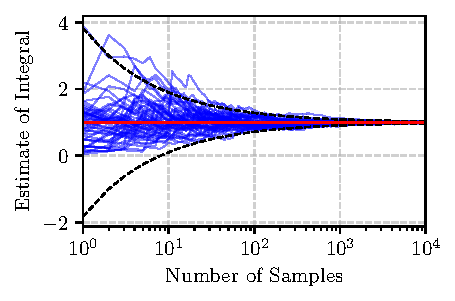
\includegraphics[width=\linewidth]{figures/numtools/monte_carlo_integration_uncorr.pdf}
    \caption{\gls{mc} estimator $\hat{I}$ using uncorrelated samples.}
    \label{fig:numtools:mc1}
  \end{subfigure}
  \begin{subfigure}[t]{0.49\linewidth}
    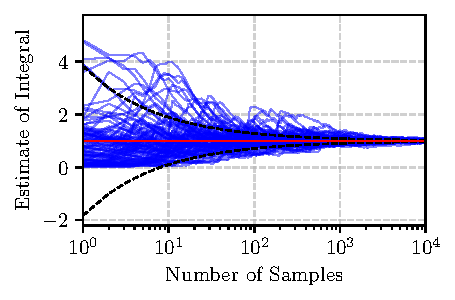
\includegraphics[width=\linewidth]{figures/numtools/monte_carlo_integration_corr.pdf}
    \caption{\gls{mc} estimator $\hat{I}$ using correlated samples with correlation length $\ell = 10$.}
    \label{fig:numtools:mc2}
  \end{subfigure}
  \caption{\gls{mc} estimation of the integral $I = \mathbb{E}[x^2]$ using uncorrelated and correlated samples. The red line represents the true value of the integral, while black dashed lines represent the theoretical $\pm 2\sigma$ confidence interval of the estimator.}
  \label{fig:numtools:mc}
\end{figure}

Fig.~\ref{fig:numtools:mc} shows the results of this experiment, using uncorrelated samples in Fig.~\ref{fig:numtools:mc1} and correlated samples in Fig.~\ref{fig:numtools:mc2}. In both cases, we see that the \gls{mc} estimator converges to the true value of the integral as $N$ increases. However, in the case of correlated samples, the variance of the estimator does not decrease as fast as in the case of uncorrelated samples, and the theoretical variance of the estimator is higher, as predicted by Eq.~\eqref{eq:ess}. 

\smallskip
This elementary example allows me to illustrate another important property of the \gls{mc} estimator, which is that the asymptotic normality of the estimator holds even for correlated samples, as long as $N \rightarrow \infty$. 

\begin{figure}[htbp]
  \centering
  \begin{subfigure}[t]{0.49\linewidth}
    \includegraphics[width=\linewidth]{figures/numtools/monte_carlo_distribution_n10.pdf}
    \caption{Distribution of the \gls{mc} estimator $\hat{I}$ using $N=10$ correlated samples.}
    \label{fig:numtools:mc3}
  \end{subfigure}
  \begin{subfigure}[t]{0.49\linewidth}
    \includegraphics[width=\linewidth]{figures/numtools/monte_carlo_distribution_n10000.pdf}
    \caption{Distribution of the \gls{mc} estimator $\hat{I}$ using $N=10,000$ correlated samples.}
    \label{fig:numtools:mc4}
  \end{subfigure}
  \caption{Histogram of the \gls{mc} estimator $\hat{I}$ using $10$ and $10,000$ correlated samples with correlation length $\ell = 10$. The red line represents the CLT approximation of the distribution of the estimator, while the histogram represents the empirical distribution of the estimator.}
  \label{fig:numtools:mc_hist}
\end{figure}

In Fig.~\ref{fig:numtools:mc_hist}, we show the empirical distribution of the \gls{mc} estimator $\hat{I}$ using $N=10$ and $N=10,000$ correlated samples with correlation length $\ell = 10$. The \gls{clt} empirical distribution of the estimator should be approximately normal with mean $I = 1$ and variance $\mathbb{V}[\hat{I}] \approx 2/N_{\mathrm{eff}}$. For $N=10$, we don't observe a normal distribution, as we have too few samples to invoke the \gls{clt}, interestingly the empirical distribution is a half-normal distribution, which is a consequence of the fact that $X^2$ is a non-negative function. However, for $N=10,000$, we see that the empirical distribution of the estimator is approximately normal, as predicted by the \gls{clt}, even in the presence of correlated samples.

\subsection{Random Walk Metropolis Algorithm for Markov Chain Monte Carlo}
\label{sec:ntools:mcmc:mcmc}

To compute the \gls{mc} estimator in Eq.~\eqref{eq:mc_estimate}, we need to be able to draw samples from the distribution $\prior{\bx}$. In the case of Bayesian inversion, this distribution is known up to a normalization constant, i.e., $\prior{\bx} = \frac{1}{\gamma} \exp{-\phi(\bx)}$, where $\phi(\bx)$ is a known potential function and $\gamma$ is an unknown normalization constant. 

\smallskip
To sample from this distribution, we can construct a Markov Chain that has $\prior{\bx}$ as its stationary distribution. A Markov Chain is a sequence of random variables $\{\bx_t\}_{t=1}^\infty$ where the distribution of $\bx_{t+1}$ depends only on the current state $\bx_t$ and not on the previous states. The transition kernel of the Markov Chain, denoted as $\mathrm{p}(\bx' \mid \bx)$, defines the probability of transitioning from state $\bx$ to state $\bx'$. We see that if the transition kernel satisfies the detailed balance condition with respect to the distribution $\prior{\bx}$, i.e.,

\begin{equation}
  \prior{\bx} \mathrm{p}(\bx' \mid \bx) = \prior{\bx'} \mathrm{p}(\bx \mid \bx')\;,
\end{equation}

then $\prior{\bx}$ is a stationary distribution of the Markov Chain. This means that if we start the Markov Chain at any initial state $\bx_0$ and let it run for a sufficiently long time, the distribution of $\bx_t$ will converge to $\prior{\bx}$ as $t \to \infty$. In practice, we usually discard the first $T_{\mathrm{burn}}$ samples of the Markov Chain, which are called the burn-in samples, and use the remaining samples.

\smallskip
Returning to our original problem, a popular algorithm for constructing a Markov Chain that satisfies the detailed balance condition with respect to the distribution $\prior{\bx}$ is the \gls{rwm} algorithm. The \gls{rwm} algorithm works as follows: given the current state $\bx_t$, we propose a new state $\bx'$ by sampling from a proposal distribution $\mathrm{q}(\bx' \mid \bx_t)$. The sample is now accepted with probability $\alpha(\bx_t, \bx')$ equal to,

\begin{equation}
  \alpha(\bx_t, \bx') = \min\left(1, \frac{\prior{\bx'} \mathrm{q}(\bx_t \mid \bx')}{\prior{\bx_t} \mathrm{q}(\bx' \mid \bx_t)}\right)\;.
  \label{eq:acceptance_probability}
\end{equation}

Eq.~\eqref{eq:acceptance_probability} defines $\mathrm{p}(\bx' \mid \bx) = \alpha(\bx, \bx') \mathrm{q}(\bx' \mid \bx)$, which can be shown to satisfy the detailed balance condition with respect to $\prior{\bx}$, and therefore $\prior{\bx}$ is a stationary distribution of the Markov Chain defined by the \gls{rwm} algorithm. A key property is that evaluating $\alpha(\bx_t, \bx')$ only requires evaluating the potential function $\phi(\bx)$ at the current and proposed states, 

\begin{equation}
  \alpha(\bx_t, \bx') = \min\left(1, \exp{-(\phi(\bx') - \phi(\bx_t))} \frac{\mathrm{q}(\bx_t \mid \bx')}{\mathrm{q}(\bx' \mid \bx_t)}\right)\;,
\end{equation}

which allows us to sample from $\prior{\bx}$ without needing to know the normalization constant $\gamma$. 
In order to guarantee that the \gls{rwm} algorithm converges, we need to choose a proposal distribution $\mathrm{q}(\bx' \mid \bx)$ that can satisfy the irreducibility condition, which states that it should be possible to reach any state $\bx'$ from any other state $\bx$ in a finite number of steps. Indeed, choosing a good proposal distribution is crucial for the efficiency of the \gls{rwm} algorithm, and is an active area of research in the \gls{mcmc} (Markov Chain Monte Carlo) literature. 

\smallskip
In this thesis, we almost exclusively use a Gaussian distribution as proposal, i.e., $\mathrm{q}(\bx' \mid \bx) = \mathcal{N}(\bx'; \bx, \mathbf{C}_{\mathrm{prop}})$. We shall discuss how to choose the covariance matrix $\mathbf{C}_{\mathrm{prop}}$ in \S\ref{sec:ntools:mcmc:advanced}.


\subsection{Convergence Diagnostics}
\label{sec:ntools:mcmc:convergence}

In practice, we need to be able to assess two fundamental questions when using \gls{mcmc} methods: (1) has the Markov Chain converged to the target distribution $\prior{\bx}$? (2) are the samples we have obtained representative of $\prior{\bx}$?. The first question is important because if the Markov Chain has not converged, then the samples we have obtained may not come from the target distribution $\prior{\bx}$ and therefore the \gls{mc} estimator may be biased. The second question is important because, as stated in \S\ref{sec:ntools:mcmc:mc}, if the samples are highly correlated, then the variance of the \gls{mc} estimator will be large and we may need to obtain more samples to achieve a good representation of the target distribution. Since each new sample from the Markov Chain depends on the previous sample, it is often the case that the samples are correlated. The amount of correlation needs to be quantified to determine the effective sample size and assess whether we have obtained enough samples to be able to reliably estimate the integral in Eq.~\eqref{eq:integral_density}.

\smallskip
\subsubsection{Convergence to the Target Distribution}

To answer whether a Markov Chain has converged to the target distribution $\prior{\bx}$, we can use the Gelman-Rubin diagnostic \cite{Gelman2013}, which is based on the idea of running multiple Markov Chains in parallel from different initial states and comparing the variance within each chain to the variance between the chains. Assume that we have $M$ Markov Chains, each of length $N$, and let $\bx_{i}^{(j)}$ be the $i$-th sample from the $j$-th chain. We can compute the within-chain variance $W$ and the between-chain variance $B$ as follows:

\begin{equation}
  \begin{aligned}
    &W = \frac{1}{N} \sum_{j=1}^{M} s_j^2\;, \text{ with }s_j^2 = \frac{1}{N-1} \sum_{i=1}^N (\bx_{i}^{(j)} - \bar{\bx}^{(j)})^2\;,\\
    &B = \frac{N}{M-1} \sum_{j=1}^{M} (\bar{\bx}^{(j)} - \bar{\bx})^2\;,
  \end{aligned}
\end{equation}

where $s_j^2$ is the sample variance of the $j$-th chain, $\bar{\bx}^{(j)}$ is the sample mean of the $j$-th chain, and $\bar{\bx}$ is the overall mean of all samples: 

\begin{equation}
  \bar{\bx} = \frac{1}{N} \sum_{j=1}^{M} \bar{\bx}^{(j)} \text{ and } \bar{\bx}^{(j)} = \frac{1}{N} \sum_{i=1}^N \bx_{i}^{(j)}\;.
\end{equation}

The Gelman-Rubin diagnostic indicator is then defined as:

\begin{equation}
  \hat{R} = \sqrt{\frac{V}{W}}\;,
\end{equation}

where $V = \frac{N-1}{N} W + \frac{1}{N} B$ is an estimate of the marginal variance of the target distribution. If the Markov Chains have converged to the target distribution, then the between-chain variance $B$ should be similar to the within-chain variance $W$, and therefore $\hat{R}$ should be close to 1. A common rule of thumb is that $\hat{R} < 1.1$ indicates convergence.

\smallskip
In this context, convergence means that the distribution of the samples from each chain is close to the target distribution $\prior{\bx}$, and that the chains are mixing well, i.e., they are exploring the target distribution effectively and the burn-in phase can be stopped.

\subsubsection{Quality of the Sample Size}

To assess how many samples we need to obtain to have a good representation of the target distribution, we can go back to the discussion in the previous section about the variance of the \gls{mc} estimator. Recalling Eq.~\eqref{eq:ess}, we see that the variance of the \gls{mc} estimator depends on the effective sample size $\neff$, which in turn depends on the correlation length $\ell$ of the samples. In practice, we rarely estimate the correlation length $\ell$ directly, but we estimate $\tau = \frac{1-\rho}{1+\rho}$, where $\rho$ is the lag-1 autocorrelation of the samples. Estimating $\tau$ allows us to compute the effective sample size as $\neff = N \tau$, and can be done directly by noting that $\tau$ is the sum of the autocorrelation function of the samples, i.e.,

\begin{equation}
  \tau = \dfrac{1-\rho}{1+\rho} = 1 + 2\sum_{k=1}^\infty \rho_k\;.
  \label{eq:ntools:tau}
\end{equation}

Where $\rho_k$ is the lag-$k$ autocorrelation of the samples. Finally, we can estimate $\hat{\rho}_k$ using the sample autocorrelation function of the samples, 

\begin{equation}
  \hat{\rho}_k = \frac{1}{N-k} \sum_{i=1}^{N-k} (f_i - \bar{f})(f_{i+k} - \bar{f})\;,
\end{equation}

where $\bar{f}$ is the sample mean of the samples. We then substitute the estimated autocorrelation function into Eq.~\eqref{eq:ntools:tau} to get an estimate of $\hat{\tau}$ but stop the summation at a certain lag $K_{\mathrm{max}}$ (computed using a heuristic such as the initial monotone sequence estimator) to avoid including noise in the estimate of $\hat{\tau}$.

\smallskip
Finally, we can use the estimate of $\hat{\tau}$ to compute the effective sample size as $\hat{N}_{\mathrm{eff}} = N \hat{\tau}$, which gives us an estimate of how many independent samples we have obtained from the Markov Chain. The desired number of samples is generally problem dependent, but it can be guided by the desired precision of the \gls{mc} estimator, which is given by $\sqrt{\mathbb{V}[\hat{I}]} = \sigma / \sqrt{\hat{N}_{\mathrm{eff}}}$.

\smallskip
If $\hat{\tau}$ is large, it means that the samples are highly correlated, and we need to obtain more samples to achieve a good representation of the target distribution. Since correlated samples are less informative than independent samples, it is often acceptable to discard a number of samples $<\ell$ to save memory. This technique is often referred to as thinning or sub-sampling.

\subsection{Example}
\label{sec:ntools:mcmc:example}

We now move to a practical example of using \gls{mcmc} methods to sample from a target distribution. We consider the problem of sampling from a mixture of two Gaussian distributions defined as follows:

\begin{equation}
  \pi(x) = 0.5\ \mathcal{N}(x; -2, 1) + 0.5\ \mathcal{N}(x; 2, 1)\;.
\end{equation}

We use a \gls{rwm} algorithm to sample from this distribution, using a Gaussian proposal distribution with variance $\sigma_{\mathrm{prop}}^2$, adapted during the burn-in phase to achieve an optimal acceptance rate of around 0.44~\cite{uq_theory}, see \S\ref{sec:ntools:mcmc:advanced} for details. We initialize the algorithm with an initial state of $x_0 = 0$ and visualize the Random Walk.

\begin{figure}[htbp]
  \centering
  \begin{subfigure}[t]{0.49\linewidth}
    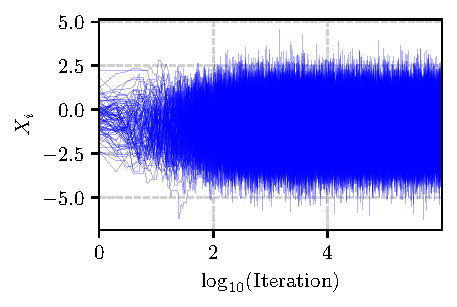
\includegraphics[width=\linewidth]{figures/numtools/mcmc_trace_paths.pdf}
    \caption{Trace plot of the Markov Chain.}
    \label{fig:numtools:mcmc_trace}
  \end{subfigure}
  \begin{subfigure}[t]{0.49\linewidth}
    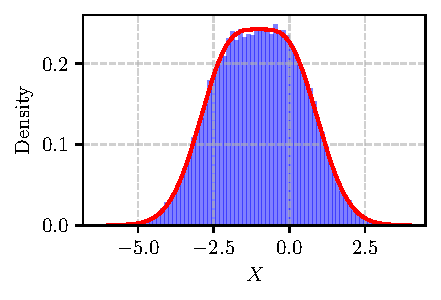
\includegraphics[width=\linewidth]{figures/numtools/mcmc_stationary_distribution.pdf}
    \caption{Histogram of the samples obtained from the Markov Chain.}
    \label{fig:numtools:mcmc_hist}
  \end{subfigure}
  \caption{MCMC sampling from a mixture of two Gaussian distributions. The trace plot shows the evolution of the Markov Chain over time, while the histogram shows the distribution of the samples obtained from the Markov Chain. The red line in the histogram represents the true distribution $\pi(x)$.}
  \label{fig:numtools:mcmc_example}
\end{figure}

Fig.~\ref{fig:numtools:mcmc_example} shows the results of this experiment. The trace plot in Fig.~\ref{fig:numtools:mcmc_trace} shows the evolution 100 \gls{rw} from the initial state $x_0 = 0$, while the histogram in Fig.~\ref{fig:numtools:mcmc_hist} shows an histogram of the steady state distribution of the Markov Chain. From Fig.~\ref{fig:numtools:mcmc_trace}, we clearly see an initial burn-in phase where the Markov Chain has not yet converged to the target distribution ($N \approx 1000$), followed by a steady state phase where the Markov Chain is exploring the target distribution. From Fig.~\ref{fig:numtools:mcmc_hist}, we see that the histogram of the samples obtained from the Markov Chain matches well with the true distribution $\pi(x)$, indicating that the Markov Chain has converged to the target distribution and that the samples are representative of $\pi(x)$.

\subsection{Advanced Topics}
\label{sec:ntools:mcmc:advanced}

In this section, we briefly discuss some advanced topics in \gls{mcmc} methods that are relevant to the work presented in this thesis and are implemented in \texttt{CMP++}. These topics include the \gls{dram} algorithm, which is an extension of the \gls{rwm} algorithm that allows for multiple proposal attempts in case of rejection and adapts the proposal covariance based on the history of the Markov Chain; the \gls{demc} algorithm, which is a population-based \gls{mcmc} algorithm that uses multiple Markov Chains to explore the target distribution and allows for interactions between the chains to improve convergence for multimodal distributions; and the \gls{hmc} algorithm, which is a gradient-based \gls{mcmc} algorithm that uses Hamiltonian dynamics to propose new states in the Markov Chain and can be more efficient than \gls{rwm} for high-dimensional target distributions.

\subsubsection{Delayed Rejection Adaptive Metropolis Algorithm}
A key parameter of the standard \gls{rwm} algorithm is the proposal covariance $\mathbf{C}_{\mathrm{prop}}$, which determines the step size of the random walk. If the proposal covariance is too small, the Markov Chain will take small steps and will mix slowly, resulting in highly correlated samples. If the proposal covariance is too large, the Markov Chain will take large steps and will have a low acceptance rate, resulting in many rejected proposals and wasted computational effort. It is known that the optimal acceptance rate for the \gls{rwm} algorithm is around 0.234~\cite{uq_theory} (at least for high-dimensional target distributions, in 1D the optimal acceptance rate is around 0.44). The target acceptance rate can be achieved by adapting the proposal covariance during the burn-in phase of the algorithm, which is the idea behind the \gls{am} algorithm. During the burn-in phase, the proposal covariance is updated based on the empirical covariance of the samples obtained so far, $\mathbf{C}_{\mathrm{prop}} = s \mathbf{C}_{\mathrm{emp}} + \epsilon \mathbf{I}$, where $s$ is a scaling factor, $\mathbf{C}_{\mathrm{emp}}$ is the empirical covariance of the samples, and $\epsilon$ is a small positive constant to ensure that the proposal covariance is positive definite. The scaling factor $s$ is updated based on the acceptance rate of the Markov Chain, with the goal of achieving the target acceptance rate,

\begin{equation}
  s^{(i+1)} = s^{(i)} \exp\left(\frac{1}{i}(\alpha^{(i)} - \alpha_{\mathrm{target}})\right)\;,
\end{equation}

where $\alpha^{(i)}$ is the acceptance rate of the Markov Chain at iteration $i$, and $\alpha_{\mathrm{target}}$ is the target acceptance rate. The \gls{dram} algorithm extends the AM algorithm by allowing for a multi-stage proposal mechanism, where if a proposal is rejected, a second proposal is generated with a different proposal covariance. The different proposal covariance can be chosen to be smaller than the original proposal covariance, $\mathbf{C}_{\mathrm{prop}}^{(2)} = \beta \mathbf{C}_{\mathrm{prop}}^{(1)}$, where $\beta < 1$ is a scaling factor (usually $\beta = 0.1$). The \gls{dram} algorithm can improve the efficiency of the Markov Chain by allowing for multiple proposal attempts in case of rejection, which can help to reduce the correlation between samples and improve the mixing of the Markov Chain.

\subsubsection{Differential Evolution Monte Carlo Algorithm}

The \gls{demc} algorithm targets multimodal distributions by using a population of Markov Chains that interact with each other to explore the target distribution. If the target distribution is multimodal, a standard proposal distribution would not be able to explore the different modes of the distribution, and the Markov Chain would get stuck in one mode. The DE-MC algorithm uses the states of the other Markov Chains in the population to propose new states for the current Markov Chain. The proposal candidate of chain $m$ at iteration $t$, $\bx'^{(m)}_t$, is generated as follows:

\begin{equation}
  \bx'^{(m)}_t = \bx^{(m)}_t + \gamma (\bx^{(m_1)}_t - \bx^{(m_2)}_t) + \eta\;,
\end{equation}

where $\bx^{(m)}_t$ is the current state of chain $m$, $\bx^{(m_1)}_t$ and $\bx^{(m_2)}_t$ are the states of two other chains $m_1$ and $m_2$ randomly selected from the population. The parameter $\gamma$ is a scaling factor that controls the step size of the proposal, and $\eta$ is a random noise term that is added to the proposal to ensure that the proposal distribution has full support. The optimal value for $\gamma$ is $\gamma = 2.38 / \sqrt{2d}$, where $d$ is the dimension of the target distribution, but every so often we set $\gamma = 1$ to allow for larger jumps in the Markov Chain. 

\subsubsection{Hamiltonian Monte Carlo (HMC) Algorithm}
In high-dimensional target distributions, the \gls{rwm} algorithm is often very inefficient, as the \gls{rw} proposal mechanism does not take into account the geometry of the target distribution, and leads to proposed jumps that are unlikely to be accepted. The \gls{hmc} algorithm is a gradient-based \gls{mcmc} algorithm that uses Hamiltonian dynamics to propose new states in the Markov Chain, which can be more efficient than \gls{rwm} for high-dimensional target distributions. 

\smallskip
To improve the quality of the proposals, we turn our random walk into a physics simulation. We assume that the log-target distribution $\log \prior{\bx}$ is a potential energy function. We then assume that the \textit{current state} $\bx$ of the Markov Chain is the initial position of a particle that is moving in such potential energy field. We then introduce a \textit{momentum} variable $\mathbf{p}$ that is independent of the position $\bx$ and is drawn from a Gaussian distribution, $\mathbf{p} \sim \mathcal{N}(\mathbf{0}, \mathbf{M})$, where $\mathbf{M}$ is a mass matrix. The Hamiltonian of the system is then defined as the sum of the potential energy and the kinetic energy, i.e.,

\begin{equation}
  H(\bx, \mathbf{p}) = -\log \prior{\bx} + \frac{1}{2} \mathbf{p}^{\top} \mathbf{M}^{-1} \mathbf{p}\;.
\end{equation}

Hamilton's equations of motion then describe how the position $\bx$ and momentum $\mathbf{p}$ evolve over time, and can be used to propose new states in the Markov Chain. The HMC algorithm uses a numerical integrator (usually the leapfrog integrator) to simulate the Hamiltonian dynamics for a certain number of steps, and then proposes the final state as the new state in the Markov Chain. The proposed state is then accepted or rejected using the Metropolis-Hastings acceptance criterion, which ensures that the Markov Chain has the correct stationary distribution.

\smallskip
The \gls{hmc} algorithm can be more efficient than \gls{rwm} for high-dimensional target distributions, as it can propose new states that are more likely to be accepted, and can explore the target distribution more effectively. However, the \gls{hmc} algorithm requires the computation of the gradient of the log-target distribution, which can be computationally expensive for complex target distributions. 

\smallskip
Furthermore, the \gls{hmc} algorithm has two hyperparameters that need to be tuned: the step size of the numerical integrator and the number of steps to simulate the Hamiltonian dynamics. If the step size is too large, the numerical integrator may not accurately simulate the Hamiltonian dynamics, leading to low acceptance rates. If the step size is too small, the Markov Chain may take a long time to explore the target distribution. The number of steps also needs to be chosen carefully, as too few steps may not allow the Markov Chain to explore the target distribution effectively, while too many steps may lead to wasted computational effort. The number of steps is usually chosen automatically using the \gls{nuts} algorithm, which ensures that the simulation stops when the trajectory starts to double back on itself (risking wasting computational effort simulating too many steps that return to the same state). The step size is usually adapted during the burn-in phase of the algorithm to achieve a desired acceptance rate (usually 0.8). The \gls{nuts} algorithm is also implemented in CMP++.



\section{Classification with Support Vector Machines}
\label{sec:ntools:svm}

In this section, we discuss the problem of classification, which is a fundamental task in machine learning and statistics. After a brief introduction to the classification problem, we focus on a specific algorithm for classification, the \gls{svm}, which is a powerful and widely used algorithm for classification tasks. We discuss the mathematical formulation of the \gls{svm}, its optimization problem, and how to use it for classification tasks. We also discuss how to extend the \gls{svm} to multi-class classification problems.


\subsection{What Is Classification?}
Similar to regression, classification is the task of learning a mapping from a set of input $\bx \in \Omega \subset \mathbb{R}^d$ to a set of discrete labels $z \in \{1, \ldots, L\}$. The difference with regression is that in classification, the output is a discrete label rather than a continuous value. We call the set of observations $\mathcal{D} = \{(\bx_i, z_i)\}_{i=1}^{\nobs}$, where $\bx_i$ is the $i$-th observation and $z_i$ is the corresponding label. 

\smallskip
Discriminative classifiers learn the conditional distribution $\mathrm{p}(z \mid \bx)$, which allows us to predict the label $z$ for a new observation $\bx$. Generative classifiers, on the other hand, learn the joint distribution $\mathrm{p}(\bx, z)$, which allows us to generate new observations $\bx$ given a label $z$. In this thesis, we focus on discriminative classifiers, which can be viewed as the task of learning a decision boundary that separates the different classes in the input space.

\begin{figure}[htbp]
\centering
% The resizebox ensures it fits perfectly on a beamer slide or fit to width
\resizebox{\textwidth}{!}{%
\begin{tikzpicture}[
    % Global aesthetic settings
    font=\sffamily,
    >=Latex,
    % Style for the connecting arrow
    connectarrow/.style={->, line width=2mm, color=gray!40, shorten >=5pt, shorten <=5pt},
    arrowlabel/.style={midway, above, font=\bfseries\large, color=black!70, align=center, yshift=5pt},
    % Clean axis style for both plots
    myaxis/.style={
        width=7cm, height=5cm,
        axis lines=left,
        % --- Remove numbers and labels ---
        xlabel={}, % Remove x-axis label
        ylabel={}, % Remove y-axis label
        xtick=\empty, % Remove x-axis ticks and numbers
        ytick=\empty, % Remove y-axis ticks and numbers
        % ----------------------------------
        ymin=-3, ymax=3,
        xmin=0, xmax=6,
        domain=0:6,
        samples=100,
        no markers,
        axis line style={-},
        % Position for legend
        legend style={font=\normalsize, at={(0.98,0.98)}, anchor=north east}
    }
]

    % Red Class (Class 1) - generally lower values
    \def\redpoints{ (1.0, 1.0) (1.5, 1.8) (2.0, 1.2) (1.2, 2.2) (1.8, 0.8) (1.0, 1.4) (2.1, 1.6) (1.3, 2.1) (1.9, 0.9) (1.6, 2.0) }
    % Blue Class (Class 2) - generally higher values
    \def\bluepoints{ (4.0, -2.0) (4.5, -1.2) (5.0, -1.8) (4.2, -0.8) (4.8, -2.2) (4.0, -1.6) (5.1, -1.4) (4.3, -0.9) (4.9, -2.1) (4.6, -1.0) }

    % Define non-linear boundary and margin coordinates (manual curves)
    % Boundary passes between red (lower y) and blue (lower y, further in x) points.
    % To have y separation, I made red positive and blue negative. 
    \def\boundary{ (0,0) (1.5,0.8) (4.5,-0.8) (6,0) }
    % Offset boundary for margins
    \def\uppermargin{ (0,0.5) (1.5,1.3) (4.5,-0.3) (6,0.5) }
    \def\lowermargin{ (0,-0.5) (1.5,0.3) (4.5,-1.3) (6,-0.5) }


    % ====== LEFT PLOT: DATA (BEFORE CLASSIFICATION) ======
    \begin{axis}[
        myaxis,
        name=dataplot,
        title={\textbf{Data Points \& Classes}},
    ]
        % Draw Red Class points with legend
        \addplot+[only marks, mark=*, mark size=3pt, mark options={fill=white, draw=red, line width=1pt}] coordinates { \redpoints };
        \addlegendentry{Class 1 (Red)};

        % Draw Blue Class points with legend
        \addplot+[only marks, mark=*, mark size=3pt, mark options={fill=white, draw=blue, line width=1pt}] coordinates { \bluepoints };
        \addlegendentry{Class 2 (Blue)};
        
    \end{axis}


    % ====== RIGHT PLOT: DISCRIMINATIVE CLASSIFIER ======
    \begin{axis}[
        myaxis,
        at={(9cm,0)}, 
        name=classifierplot,
        title={\textbf{Discriminative Classifier \& Boundary}},
    ]
        % Replicate Data Points
        \addplot+[only marks, mark=*, mark size=3pt, mark options={fill=white, draw=red, line width=1pt}] coordinates { \redpoints };
        \addplot+[only marks, mark=*, mark size=3pt, mark options={fill=white, draw=blue, line width=1pt}] coordinates { \bluepoints };

        % Boundary Plot
        \addplot[black, thick, smooth, tension=0.7] coordinates { \boundary };

        % Margin Plots
        \addplot[black, dashed, smooth, tension=0.7] coordinates { \uppermargin };
        \addplot[black, dashed, smooth, tension=0.7] coordinates { \lowermargin };
        
    \end{axis}


    % ====== CONNECTING ARROW ======
    % Draw arrow between the two axis environments
    \draw[connectarrow] ($(dataplot.east)+(0.2,0)$) -- 
                        node[arrowlabel] {} 
                        ($(classifierplot.west)+(-0.2,0)$);

\end{tikzpicture}
} % End resizebox
\caption{Illustration of the classification problem. The left plot shows a set of observations (data points) belonging to two different classes (red and blue). The right plot shows a discriminative classifier that learns a decision boundary (solid black line) that separates the two classes, along with the margins (dashed lines) that define the region of uncertainty around the decision boundary.}

\label{fig:classification_problem}
\end{figure}

Fig.~\ref{fig:classification_problem} illustrates the classification problem. The left plot shows a set of observations (data points) belonging to two different classes (red and blue). The right plot shows a discriminative classifier that learns a decision boundary (solid black line) that separates the two classes, along with the margins (dashed lines) that define the region of uncertainty around the decision boundary. 

\smallskip
When dealing with classification problems, we often encounter situations where the classes are not linearly separable in the input space. Finding non-linear decision boundaries is often impractical, as those are often complex and difficult to generalize. Instead, we can expand the input space into a higher-dimensional feature space, where the classes may become linearly separable. This is the idea behind kernel methods, which define a mapping from the input space to a higher-dimensional feature space, where a linear decision boundary can be learned. The Support Vector Machine (SVM) is a powerful algorithm that uses a \textit{trick}, called the kernel trick, to implicitly map the input space into a higher-dimensional feature space, without increasing the computational complexity of the algorithm.

\subsection{Support Vector Classification}
A \gls{svc} is a discriminative classifier that constructs a hyperplane to optimally separate the classes. To deal with non-linearly separable classes, the \gls{svc} uses the kernel trick to implicitly map the input space into a higher-dimensional feature space where a linear separation is possible. The \gls{svc} finds the hyperplane that maximizes the margin between the classes in this feature space, which leads to good generalization performance on unseen data.

\begin{figure}[htbp]
  \centering
  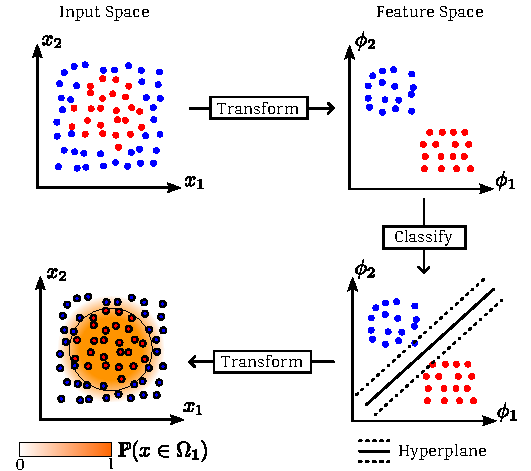
\includegraphics[width=0.6\linewidth]{figures/clustering/classify.pdf}
  \caption{A schematic representation of the \gls{svm} classification process with the transformation of the input into the feature space. }
  \label{fig:SVM_classification}
\end{figure}

Fig.~\ref{fig:SVM_classification} illustrates the \gls{svm} classification process and the transformation of the input into the feature space.

\smallskip
Note that the \gls{svc} is a binary classifier, which means that it can only separate two classes at a time. We shall later see how to extend the \gls{svc} to multi-class classification problems. For now, we focus on the binary classification case, where we have two classes $\{1,2\}$, and we want to learn a hyperplane that separates the two classes in the feature space. To pass from the input space to the feature space, we use a covariance function $k_{\bpsi}(\bx, \bx')$ that defines the inner product in the feature space, i.e., $\langle \boldsymbol{\phi}(\bx), \boldsymbol{\phi}(\bx') \rangle = k_{\bpsi}(\bx, \bx')$, where $\boldsymbol{\phi}(\cdot)$ is the implicit mapping from the input space to the feature space. The equation of the hyperplane in the feature space can be written as follows,

\begin{equation}
  f(\bx) = \mathbf{w}^{\top} \bphi(\bx) + \mathrm{b}\;,
  \label{eq:decision_function}
\end{equation}

where $\mathbf{w}$ is a set of coefficients that define the hyperplane and $\mathrm{b}$ is the bias term, the hyperplane is defined as the set of points $\bx$ such that $f(\bx) = 0$. In practice, we never explicitly compute the mapping $\boldsymbol{\phi}(\cdot)$ or the coefficients $\mathbf{w}$, because the dimensionality of the feature space would be massive. Instead, we can express the optimal weights $\mathbf{w}$ as a linear combination of the training observations in the feature space, i.e., $\mathbf{w} = \bphi(\mathbf{X})^{\top} \mathbf{Y} \boldsymbol{\alpha}$, where $\mathbf{X}$ is the matrix of training observations, $\mathbf{Y}$ is a diagonal matrix (containing +1 or -1 depending on the class labels), and $\boldsymbol{\alpha}$ is a vector of Lagrange multipliers. Substituting this expression for $\mathbf{w}$ into Eq.~\eqref{eq:decision_function}, we get:

\begin{equation}
  f(\bx) = \boldsymbol{\alpha}^{\top} \mathbf{Y} \bphi(\mathbf{X}) \bphi(\bx) + \mathrm{b} = \boldsymbol{\alpha}^{\top} \mathbf{Y} k_{\bpsi}(\mathbf{X}, \bx) + \mathrm{b}\;.
  \label{eq:decision_function_kernel}
\end{equation}

We now have an expression for the decision function in terms of the kernel function, which allows us to compute the decision function without explicitly computing the mapping $\boldsymbol{\phi}(\cdot)$ to the feature space. This is known as the kernel trick and is a key feature of SVMs that allows them to efficiently handle high-dimensional feature spaces, without increasing the size of the vector of Lagrange multipliers $\boldsymbol{\alpha}$. 

\smallskip
Notice that in this context, the kernel function $k_{\bpsi}(\bx, \bx')$, although interpreted differently, is actually the same as the covariance function used in \gls{gpr} since they both satisfy the properties of a positive semi-definite function. In this work we shall use the word kernel to refer to the covariance function in the context of \gls{svm} and the word covariance to refer to the covariance function in the context of \gls{gpr}. The reader shall not confuse the \gls{svc} \textit{kernel} with the \textit{kernel} used in \gls{kde}, as the latter is a positive function of a distance metric that integrates to one. To estimate the parameters $\boldsymbol{\alpha}, \mathrm{b}$, we can use the training data and solve the following optimization problem:

\begin{equation}
  \left.
  \begin{aligned}
    &\min_{\boldsymbol{\alpha}} \frac{1}{2} \boldsymbol{\alpha}^{\top} \mathbf{Y} k_{\bpsi}(\mathbf{X}, \mathbf{X}) \mathbf{Y} \boldsymbol{\alpha} - \sum_{i=1}^{\nobs} \alpha_i\;.\\
    &\text{s.t. } \left\{
    \begin{aligned}
      &\sum_{i=1}^{\nobs} \alpha_i y_i = 0\\
      &0 \leq \alpha_i \leq \mathrm{C}
    \end{aligned}
    \right.
  \end{aligned}
  \right.
\end{equation}

where $\mathrm{C}$ is a regularization parameter that controls the trade-off between maximizing the margin and minimizing the classification error on the training data. The optimization problem can be solved using quadratic programming techniques, and the resulting parameters $\boldsymbol{\alpha}, \mathrm{b}$ can be used to compute the decision function for any new input $\bx$~ \cite{libsvm}.


\smallskip
The theory presented here is valid only for the binary classification case; to actually perform multi-class classification, we need to use a strategy to combine multiple binary classifiers~\cite{multi_class_classification}. A common strategy is the \gls{ovr} strategy, where we train $L$ binary classifiers, each one trained to separate one class from the rest. The decision function for a new input $\bx$ is then computed as the maximum of the decision functions of the $L$ binary classifiers, i.e.,

\begin{equation}
  f(\bx) = \arg\max_{l=1\ldots L} \left( \boldsymbol{\alpha}_l^{\top} \mathbf{Y}_l k_{\bpsi}(\mathbf{X}, \bx) + \mathrm{b}_l \right)\;.
\end{equation}

This strategy is simple and effective for many applications and it can handle many classes. An alternative strategy is the \gls{ovo} strategy, where we train a binary classifier for each pair of classes, resulting in $L(L-1)/2$ binary classifiers. The decision function for a new input $\bx$ is then computed using a voting scheme, where each binary classifier votes for one of the two classes it was trained on, and the class with the most votes is selected as the final prediction. Although the \gls{ovo} strategy requires more binary classifiers than the \gls{ovr} strategy, it is generally more accurate and requires less training data for each binary classifier, since each binary classifier only needs to distinguish between two classes rather than one class and the rest~\cite{libsvm}.

\subsection{Probability Estimates}
\label{sec:ntools:svm:probability}

The decision function of the \gls{svm}, given by Eq.~\eqref{eq:decision_function_kernel}, provides a score that indicates how far an input $\bx$ is from the decision boundary. However, this function has a co-domain of $\mathbb{R}$, which makes it difficult to interpret the output as a probability. 

\smallskip
Indeed, we would like to have a probabilistic interpretation of the output of the \gls{svm}, where the output represents the probability that a given input $\bx$ belongs to a certain class. We denote this probability as $\mathbb{P}_{\mathrm{SVC}}(\bx \in \Omega_l) \text{ s.t. } \sum_{l=1}^L \mathbb{P}_{\mathrm{SVC}}(\bx \in \Omega_l) = 1$, which represents the probability that the input $\bx$ belongs to class $l$ according to the SVC (or equivalently, the probability that $\bx$ belongs to the subdomain $\Omega_l$).

\smallskip
To obtain probability estimates from the \gls{svc}, we can use a technique called Platt scaling~\cite{platt_2000,lin_2003}. The basic idea behind Platt scaling is that, in a \gls{ovo} setting, the decision function of each binary classifier can be passed through a sigmoid function to obtain a probability estimate for the binary classification problem. Specifically, for each binary classifier that separates class $l$ from class $m$, we can compute the probability that an input $\bx$ belongs to class $l$, $\mathbb{P}_{\mathrm{SVC}}(\bx \in \Omega_l \mid \bx \in \Omega_l \cup \Omega_m)$, as follows:

\begin{equation}
  \mathbb{P}_{\mathrm{SVC}}(\bx \in \Omega_l \mid \bx \in \Omega_l \cup \Omega_m) = \frac{1}{1 + \exp{(A f_{lm}(\bx) + B)}}\;,
\end{equation}

where $A$ and $B$ are parameters that can be estimated via \gls{cv} on the training data, and $f_{lm}(\bx)$ is the decision function of the binary classifier that separates class $l$ from class $m$~\cite{libsvm}. Of course, we would like to have a single probability estimate for each class, rather than one for each pair of classes. To achieve this, we note that,

\begin{equation}
\begin{split}
  &\mathbb{P}_{\mathrm{SVC}}(\bx \in \Omega_m \mid \bx \in \Omega_l \cup \Omega_m) \mathbb{P}_{\mathrm{SVC}}(\bx \in \Omega_l) = \\
  & \mathbb{P}_{\mathrm{SVC}}(\bx \in \Omega_l \mid \bx \in \Omega_l \cup \Omega_m) \mathbb{P}_{\mathrm{SVC}}(\bx \in \Omega_m)\;,
\end{split}
\end{equation}

which is just a restatement of Bayes' theorem. Since the probabilities $\mathbb{P}_{\mathrm{SVC}}(\bx \in \Omega_l)$ are unknown, we can use the above equation (which must hold for all pairs of classes) to set up an optimization problem to solve for the probabilities $\mathbb{P}_{\mathrm{SVC}}(\bx \in \Omega_l)$~\cite{libsvm,wu_2004}.


\subsection{Hyperparameter Selection}
\label{sec:ntools:svm:hyperparameter}

The performance of the \gls{svc} depends on the choice of hyperparameters, which are parameters that are not learned from the training data but rather set by the practitioner. The main hyperparameters of the \gls{svc} are the regularization parameter $\mathrm{C}$ and the parameters of the kernel function $k_{\bpsi}(\cdot, \cdot)$, usually a simple correlation length $l$ that controls the width of the kernel. The regularization parameter $\mathrm{C}$ controls the trade-off between maximizing the margin and minimizing the classification error on the training data. A small value of $\mathrm{C}$ allows for a larger margin but may lead to more misclassifications, while a large value of $\mathrm{C}$ leads to a smaller margin but fewer misclassifications. The choice of hyperparameters can have a significant impact on the performance of the SVC, and it is important to select them carefully.

\smallskip
The authors of \texttt{LIBSVM}~\cite{libsvm}, given the small number of hyperparameters, suggest performing a grid search over a predefined set of $\mathrm{C}$ and $\gamma$ values, and selecting the combination that yields the best predictive accuracy (e.g., classification accuracy on a validation set or using \gls{cv}). The grid search approach is simple and effective, but is computationally expensive, especially for large datasets or when the number of hyperparameters is large.


\smallskip
To improve upon grid search and cross-validation, Vapnik and Chapelle demonstrated that the \gls{loo} error, an unbiased estimator of the performance of the \gls{svc}, can be bounded by a quantity called the geometric span~\cite{chapelle_2002}. The theorem states that if a point $x_i$ is a free support vector (lying exactly on the margin, $0 < \alpha_i < C$), its \gls{loo} classification status is dictated by its dual coefficient $\alpha_i$ and its geometric span $S_i^2$. The span $S_i^2$ represents the distance in the feature space between $x_i$ and the affine subspace spanned by the remaining support vectors.

\smallskip
The geometric span for each free support vector $i$ is extracted directly from the diagonal of the inverted matrix,

\begin{equation}
    S_i^2 = \frac{1}{[\mathbf{Q}^{-1}]_{ii}} \;.
\end{equation}

where $\mathbf{Q} = \mathbf{Y} k_{\bpsi}(\mathbf{X},\mathbf{X}) \mathbf{Y}$. The span $S_i^2$ quantifies how much influence each free support vector has on the decision boundary, with larger spans indicating that the point is more critical to the classification decision. The \gls{loo} error can then be bounded by the sum of the products of the dual coefficients and the geometric spans of the free support vectors, plus the number of bounded support vectors $\mid S_B \mid$ (those that lie inside the margin, $\alpha_i = C$), which are always misclassified in the \gls{loo} procedure:

\begin{equation}
  \mathcal{E}_{\mathrm{LOO}} \leq \sum \alpha_i S_i^2 + \mid S_B \mid \;,
  \label{eq:span_loo}
\end{equation}

\smallskip
By minimizing Eq.~\eqref{eq:span_loo} with respect to the hyperparameters, we can improve the generalization performance on unseen data. In practice, Eq.~\eqref{eq:span_loo} is minimized using the \texttt{NLopt} library~\cite{nlopt}, which implements a variety of optimization algorithms, including global and local optimization methods.

